\chapter{Asking Wealthy Americans How They Got Rich! (Florida)}

This lecture is built out of street interviews, but its internal logic is more deliberate than that format first suggests. We begin with consequences before causes, widen to Tampa as a dense field of wealth, and then let the city yield a sequence of cases: people before homogenization, diversification across categories, leverage as a capital instrument, time as the scarce asset, self as brand, living beneath means, and finally the sharp distinction between paying with time and paying with creativity. No validated board frame survives from this lecture, so the mathematics here is transcript-led and intentionally cautious: whenever we write formulas, we are cleaning up the commercial logic already present in the spoken lecture.

\section{Cold Open and Tampa as a Wealth Field}

The lecture opens by spending outcome before mechanism. We hear fragments of later payoff and later risk before the city has even been named:
\begin{equation}
Y_{\text{teaser},1} > \$10\,\text{million},\qquad
Y_{\text{teaser},2} \approx \$15\,\text{million},\qquad
L_{\text{teaser}} = \$550{,}000.
\end{equation}
This is not yet an argument. It is a promise. The lecture wants us to feel scale first and only then ask how that scale was produced.

There is also an unstable money fragment in the teaser that sounds like \(\$45\) million. Later coherent speech, however, strongly suggests that the intended current-year figure in that later case is
\begin{equation}
Y_{\text{digital,current}} \approx \$4\text{--}5\,\text{million/year},
\end{equation}
so we should not build the chapter on the teaser splice alone.

Only after that does the host tell us why Tampa is the chosen field:
\begin{equation}
N_{\text{millionaires}} > 60{,}000,\qquad
N_{\text{billionaires}} \approx 10.
\end{equation}
These are not used as data to be proved. They are used to justify the method. If a city has wealth at that density, then walking through its expensive districts and stopping operators becomes, in the lecture's logic, a way of extracting rules from the field itself.

The host then states the mission plainly: we are going to move through Tampa, find people who have built serious businesses, and ask how they became financially free. That framing matters, because it means that everything that follows will oscillate between anecdote and doctrine. The lecture will repeatedly ask us to move from a person, to a number, to a mechanism.

\section{The Older Serial Entrepreneur: People, Diversification, and the Cash Call}

The first long case belongs to an older entrepreneur who says he has been an entrepreneur his whole life. The striking thing is that the lecture does not begin with his revenue. It begins with his management doctrine. He was in television; he was in restaurants; and the great lesson he draws from business is not at first financial at all: take care of your people. Once a larger corporation buys the company and tries to homogenize everything, he says, the machine breaks because the new owners do not care about staff in the same way.

That is the first structural lesson of the chapter. The lecture wants us to see that the business can be large and still be governed by a human variable. Only then does it give us the scale markers:
\begin{equation}
R_{\text{TV}} \approx \$30\text{--}40\,\text{million/year},\qquad
R_{\text{restaurant}} \approx \$5\,\text{million/year}.
\end{equation}
Again, we should keep these as revenues, not personal income. The lecture is speaking here about the scale of the operating businesses.

He then adds the second major rule. He tried always to have
\begin{equation}
N_{\text{income sources}} = 3
\end{equation}
and, crucially, not three copies of the same business. The point is categorical separation:
\begin{equation}
\{\text{television},\ \text{restaurant},\ \text{farming}\},
\qquad
\text{category}_1 \neq \text{category}_2 \neq \text{category}_3.
\end{equation}
This is not the modern startup injunction to concentrate every unit of energy on one product. It is a different logic: if one sector stalls, the others may continue to produce.

\subsection{Question \& Answer}

\paragraph{Question.} Why diversify across distinct businesses if many entrepreneurs preach concentration?

\paragraph{Answer.} Because the lecture is describing a portfolio logic, not an early-stage startup logic. The older entrepreneur is not telling us to scatter our attention randomly. He is telling us that once we are building durable wealth, it is dangerous to let all risk remain correlated. In the language of the lecture, television, restaurants, and farming are not merely three businesses; they are three different failure modes. That is why the chapter should preserve this as a distinct line of reasoning rather than flatten it into generic advice about ``multiple streams.''

The interview then turns from diversification to biography. He says he grew up on a farm, and when asked about the turning point to financial freedom, he points back toward his father, who took risk every day. The lecture is making a quiet move here. It is telling us that appetite for risk is not being narrated as a personality trick. It is being narrated as inheritance, environment, and example.

There is also an age marker:
\begin{equation}
a_{\text{older}} \approx 69,\qquad
a_{\text{older,next year}} = 70.
\end{equation}
The host reacts with surprise, and this matters narratively. Age here is used to add authority to the advice that follows.

That next advice is one of the clearest business screens in the lecture. When a venture needs fresh liquidity, he says, the partners must be able to answer ``the call'':
\begin{equation}
\text{good partner} \;\Rightarrow\; \text{can meet cash call } C,
\qquad
\text{cannot meet } C \;\Rightarrow\; \text{not a viable partner}.
\end{equation}
This is not formal corporate-finance language. It is operator language. But it is precise enough to retain. The partner is being tested not by personality, not by shared enthusiasm, but by capacity under pressure.

The same interview closes with an older-credit-world anecdote that the lecture had already teased at the beginning. He says he once walked into a bank on a Saturday, met the bank president on his day off, and secured
\begin{equation}
L_{\text{first business}} = \$550{,}000
\end{equation}
to open his first business. The point is not nostalgia for easy money. The point is that finance, partnership, and diversification are all being presented as parts of one operating picture.

When the host steps back from this interview, he compresses the whole thing into a social rule: attach ourselves to great people, because people will take us places money cannot. That recap is essential. It turns the entire first case from biography into doctrine before the lecture moves on.

\section{The Younger Investor: Leverage Debt and Choose Your Hard}

The next major case changes the temperature. The speaker is much younger, runs a digital-marketing company, and says he has been an entrepreneur for only about
\begin{equation}
T_{\text{digital}} \approx 3\text{--}4\ \text{years}
\end{equation}
while already making roughly
\begin{equation}
Y_{\text{digital,current}} \approx \$4\text{--}5\,\text{million/year}.
\end{equation}
The lecture now pivots away from the earlier emphasis on people and diversification and toward capital structure.

His doctrine comes fast: leverage debt. The point, as he phrases it, is that many people are obsessed with escaping debt, but that merely moving from negative to zero is not yet wealth creation. In a cleaned companion-note form, we may write
\begin{equation}
W<0 \;\to\; W=0
\end{equation}
as debt elimination without actual asset creation.

What he wants instead is a machine in which borrowed capital acquires a cash-flowing asset. The cleanest note-writer diagram is the following transcript-derived schematic:

\begin{figure}[h]
\centering
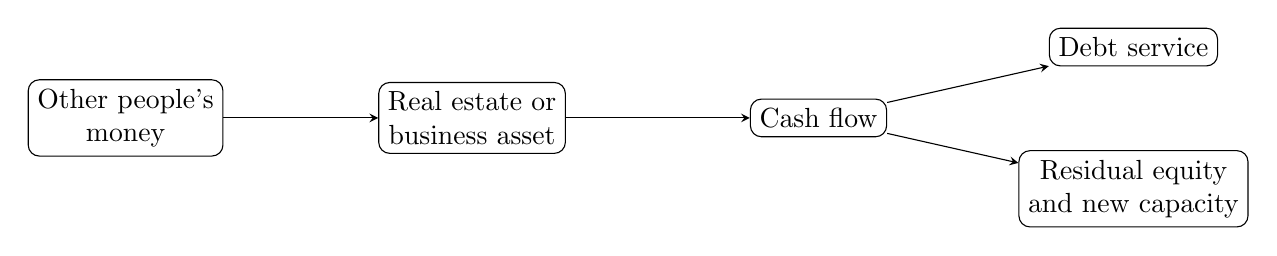
\begin{tikzpicture}[>=stealth]
\node[draw, rounded corners, align=center] (a) at (0,0) {Other people's\\money};
\node[draw, rounded corners, align=center] (b) at (4.4,0) {Real estate or\\business asset};
\node[draw, rounded corners, align=center] (c) at (8.8,0) {Cash flow};
\node[draw, rounded corners, align=center] (d) at (12.8,0.9) {Debt service};
\node[draw, rounded corners, align=center] (e) at (12.8,-0.9) {Residual equity\\and new capacity};
\draw[->] (a)--(b);
\draw[->] (b)--(c);
\draw[->] (c)--(d);
\draw[->] (c)--(e);
\end{tikzpicture}
\caption{Transcript-derived leverage loop from the younger entrepreneur's explanation.}
\end{figure}

In symbolic form, the same idea may be written as
\begin{equation}
\text{OPM}
\;\to\;
\text{asset purchase}
\;\to\;
\text{cash flow}
\;\to\;
\text{debt repayment}.
\end{equation}
Here \(\text{OPM}\) is only shorthand for ``other people's money.'' It is not spoken as notation in the lecture.

We can push the logic one step further without leaving the speaker's meaning. Let \(F\) denote periodic cash flow from the acquired asset and \(D\) periodic debt service. Then the mechanism he has in mind is viable only if
\begin{equation}
F>D.
\end{equation}
In that case, the simplest update rule for retained wealth is
\begin{equation}
W_{n+1}=W_n + (F-D).
\end{equation}
This is not the speaker's algebra. It is our cleaned form of what he means when he says that borrowed money can start something which then pays the debt back over time.

\subsection{Question \& Answer}

\paragraph{Question.} How can debt function as a wealth-building tool rather than merely as a liability?

\paragraph{Answer.} In the lecture's own logic, debt becomes a tool only when it sits in front of an asset that throws off cash flow. If borrowing merely funds consumption, it is dead weight. If borrowing funds a property or business whose inflow exceeds its debt service, then the debt is acting as an accelerant. That is why the speaker is so emphatic: without learning how to use leverage, one remains employed by people who already know how to do exactly that.

The lecture then protects this doctrine from sounding too cold or purely technical by widening into biography. The speaker says he went to college for only
\begin{equation}
T_{\text{college}} \approx 90\ \text{days},
\end{equation}
left quickly, and became a millionaire at about
\begin{equation}
a_{\text{millionaire}} \approx 27.
\end{equation}
He also describes severe instability in childhood: father dead very early, mother jailed for a period. The lecture is doing something important here. It is refusing to let leverage appear as a trick available only to the already comfortable. It is embedding the doctrine inside hardship.

That is why the section ends not on debt, but on a maxim:
\begin{equation}
\text{hard}_{\text{build/invest/repair}}
\qquad \text{vs.} \qquad
\text{hard}_{\text{stay broke/stagnate}}.
\end{equation}
The lecture's point is not that business is easy. It is that hardship is unavoidable; what matters is which hardship we are willing to bear.

\section{Sponsor Interruption: Time as the Scarce Asset}

At this point the lecture interrupts itself. The host says that one of the greatest lessons learned from interviewing many wealthy people is that time is the one asset we never get back. That is the real bridge into the sponsor block.

The sponsor arithmetic is simple and should remain structurally separate from the main interview logic:
\begin{equation}
N_{\text{millionaires interviewed}} > 1000,\qquad
d_{\text{CookUnity}} = 50\%.
\end{equation}
Later, just before the Bautista interview, the host also gives channel scale numbers:
\begin{equation}
N_{\text{followers}} = 8\,\text{million},\qquad
V_{\text{monthly views}} \approx 170\,\text{million/month}.
\end{equation}
This is not the same kind of mathematics as the earlier business doctrine. It is the arithmetic of attention, scale, and promotional pricing. But the transition is not random. The host is monetizing the claim that time is scarce by pointing to a convenience product that supposedly frees time for business building.

We should therefore preserve the interruption, but not let it swallow the chapter. It is a hinge, not the spine.

\section{David Bautista: Commodity, Brand, and Living Beneath Means}

The next case changes the register again. We now move into entertainment, but the lecture does not abandon business reasoning. David Bautista says he has been in the entertainment business for about
\begin{equation}
T_{\text{Bautista,entertainment}} \approx 25\ \text{years}
\end{equation}
and has made more than
\begin{equation}
Y_{\text{Bautista,max}} > \$10\,\text{million/year}.
\end{equation}
But he immediately pairs that scale with a much harsher origin story: single mother, periods without enough food, the worst parts of Washington, D.C., and no real money until well into his thirties:
\begin{equation}
T_{\text{Bautista,no money}} \approx \text{until well into his 30s}.
\end{equation}
Again the lecture refuses to let the endpoint float free of the path.

The first mentor doctrine comes from Triple H. Bautista says he was initially too worried about hierarchy, about disrespect, about making enemies. The lesson he retains is that he must treat himself as a business. In compact note form:
\begin{equation}
\text{self} = \text{business} = \text{commodity} = \text{brand}.
\end{equation}
This is not metaphysics. It is commercial framing. The lecture wants us to see that once the self becomes a revenue-producing object, decisions about reputation, behavior, and positioning must be treated structurally rather than emotionally.

The second doctrine comes from The Undertaker, who tells him to live beneath his means. In the simplest mathematical form:
\begin{equation}
C<Y,\qquad S=Y-C>0,
\end{equation}
where \(C\) is consumption, \(Y\) income, and \(S\) retained surplus. That is the cleanest note form of the rule.

We can make the logic one step more explicit. If the surplus \(S\) is maintained year after year, and if we ignore returns for the moment, then the wealth path satisfies
\begin{equation}
W_n = W_0 + nS.
\end{equation}
This small formula is enough to capture the lecture's commercial point. A person who lives beneath his means is not merely being ``responsible.'' He is creating an update rule under which time works in his favor.

\subsection{Question \& Answer}

\paragraph{Question.} Why does living beneath one's means remain rational even after very large earnings?

\paragraph{Answer.} Because the lecture is not treating high income as the same thing as durable wealth. Bautista explicitly says he learned this the hard way. He lost everything after wrestling, his house was foreclosed on, and the second opportunity in film arrived only afterward. Once we understand that sequence, the rule \(C<Y\) stops sounding moralistic and starts sounding structural. The money in the bank is worth more than one more unnecessary object because stored optionality is what makes the next reinvention possible.

This is also why the Bugatti example matters:
\begin{equation}
P_{\text{Bugatti}} \approx \$3\text{--}5\,\text{million}.
\end{equation}
He does not say the car is evil. He says he does not need it. That distinction is important. The lecture is not anti-pleasure. It is anti-confusing wants with durable position.

The section then ends on an even harsher piece of business realism. Entertainment, he says, is a machine. We do not necessarily have to like everyone with whom we do business. If someone can generate money for us, or we for them, that is enough to sustain a working relation. The lecture had earlier raised the question of being liked; now it answers it by subordinating likability to commercial usefulness.

When the host recaps the interview, he sharpens this further: if we go into business trying to please everyone, we will not be successful. That recap matters because it turns Bautista's segment from celebrity color into doctrine and prepares the final move of the lecture.

\section{The Final Consultant: Paying with Time, Paying with Creativity}

The last long case resolves the opening teaser. We return to the consultant in the Rolls Royce, now in full form. He says he has been a business owner for
\begin{equation}
T_{\text{final consultant}} = 39\ \text{years},
\end{equation}
and that the most money he has ever made in a single year is about
\begin{equation}
Y_{\text{final,max}} \approx \$15\,\text{million/year}.
\end{equation}
Asked whether he has been broke, he answers with a sequence rather than a single event:
\begin{equation}
W_{\text{broke}}
\to
W_{\text{millions}}
\to
W_{\text{broke again}}
\to
W_{\text{stabilized}}.
\end{equation}
This is a good closing structure for the lecture, because it ties together the earlier recurring theme that large incomes do not by themselves end financial vulnerability.

He then gives the lecture's most abstract wealth distinction. Poor and middle-class people, he says, feel that things are expensive because they pay for them with money exchanged directly for time, and therefore with life itself. Wealthy creative entrepreneurs pay in a different currency. In compact form:
\begin{equation}
\text{purchase}_{\text{poor/middle}}
\sim t_{\text{labor}},
\qquad
\text{purchase}_{\text{wealthy entrepreneur}}
\sim c_{\text{creative offer}}.
\end{equation}
This is not a theorem of literal prices. The speaker is obviously not claiming that market prices disappear. He is distinguishing two mechanisms of payment. One sells hours first and buys later. The other creates an offer, a structure, a piece of commercial creativity, and uses that to finance the purchase.

\subsection{Question \& Answer}

\paragraph{Question.} What does it mean to pay for things with creativity rather than with time?

\paragraph{Answer.} It means that the entrepreneur is not simply converting labor hours into wages and wages into purchases. He is creating an offer, a structure, or a commercial situation that generates the means of payment. In the lecture's language, the poor and middle class pay with time, while the creative operator pays with invention. We should keep this speaker-attributed and heuristic. It is a sharp distinction, but not a literal identity saying that all prices are numerically equal.

The lecture then makes one final turn, from commercial abstraction back into spiritual ordering. The consultant says he does not merely believe in God; he trusts God. He received Christ at
\begin{equation}
a_{\text{received Christ}} = 16,
\end{equation}
started reading the Bible at
\begin{equation}
a_{\text{began Bible reading}} = 17,
\end{equation}
and says that whenever he learns a success principle, he checks whether it aligns with Scripture. If it does, he follows it; if not, he discards it. The lecture ends, then, not with a spreadsheet but with a filter. Even the wealth doctrine must answer to a higher criterion.

\section{Summary}

The lecture begins by showing us outcomes before it tells us what produced them, and that choice is not cosmetic. It allows Tampa to appear as a field charged with wealth before the cases begin to explain it. Once the city is set, the lecture proceeds through a disciplined sequence: people before homogenization, diversification across distinct categories, partner quality measured by the cash call, leverage debt as a way of using someone else's money to acquire cash-flowing assets, time as the irrecoverable resource, self as business and brand, living beneath means as an update rule rather than a moral slogan, and finally creativity as a higher payment mechanism than labor-time alone.

What ties these segments together is not one universal formula, but a repeated movement from surface sign to underlying mechanism. A Rolls Royce is not the lesson; the capital structure is. Celebrity is not the lesson; brand discipline and restraint are. High income is not the lesson; retained optionality is. If we keep that progression visible, then the chapter remains faithful to the lecture's actual rhythm: from anecdote, to number, to rule, and then onward to the next search.